\chapter{Bosón $W$}\label{Ch:W}
En el año 1933, Fermí presenta al mundo su teoría original de la desintegración beta~\cite{Fermi:1933jpa}, en esta los procesos son tratados como interacciones de contacto, las cuales se producen en un único punto, es decir, no se requiere de partículas intermediarias. Debido a que la interacción débil (la responsable de la desintegración beta) es de muy corto alcance, la suposición propuesta por Fermí es acertada y produce excelentes resultados a bajas energías. Sin embargo, debido a los desarrollos teóricos de la época se sabía que a altas energías esta aproximación no era útil y por lo tanto se debía crear una teoría en la cual la interacción estuviera mediada por alguna partícula. Algunos físicos teóricos propusieron una partícula intermediaría que llamaron bosón  vectorial intermediario~\cite{Lee:1960qw}. A partir de allí el desafío para lo físicos teóricos era predecir las propiedades del bosón vectorial intermediario, y para los experimentales, producir este en el laboratorio.
Debido a que no había un modelo o teoría que diera información formal sobre el bosón vectorial intermediario, las conjeturas sobre su masa se fueron refinando a medida que los experimentos aumentaban progresivamente la energía. En 1965 se creía que la masa debía ser al menos masa del protón~\cite{Kienzle:1965zz}; 10 años después, el límite inferior experimental creció a $2.5$ veces la masa del protón~\cite{Kramer:1970ed}. Sin embargo, fue necesario esperar hasta la aparición de la teoría electrodébil de Glashow, Weinberg y Salam. Esta teoría daba argumentos firme sobre el valor de dicha masa. De hecho, en esta teoría hay tres bosones vectoriales intermedios, dos de ellos cargados ($W^{\pm}$) y uno neutral ($Z$). Las predicciones dadas por la teoría electrodébil establecía que las masas de estos bosones vectoriales intermedios debía ser~\cite{Weinberg:1967tq}:
\begin{align}
M_{W} =& 82 \pm 2 \text{ GeV/c}^2\,, & M_{Z} =& 92 \pm 2 \text{ GeV/c}^2\,.
\end{align}

De la teoría electrodébil se conocía que todos los hadrones y leptones participan en la interacción débil, pero debido a que dicha interacción solo es relevante en ausencia de las interacciones fuertes y electromagnéticas, la masa de estos bosones vectoriales intermediarios es difícil de medir. La dificultad fue superada debido a la construcción del colisionador protón-antiprotón Super Proton Synchrotron (SPS, supersincrotrón de protones) del CERN~\cite{Arnison:1983mk, Arnison:1983rp}, mediante el cual fue posible producir estas partículas extremadamente pesadas (la masa del protón es de $1 \text{ GeV/c}^2$, por lo que estos bosones vectoriales intermediarios son casi $100$ veces más pesados que el protón). En enero de 1983, el grupo de Carlo Rubbia informó sobre el descubrimiento de los $W$ (a $81.5\text{ GeV/c}^2$) y en junio, el mismo grupo anunció el descubrimiento del $Z$ (a $95.3 \text{ GeV/c}^2$)~\cite{Rubbia:1984xy}. Esto significo un extraordinario triunfo técnico y de fundamental importancia para la comunidad de física, ya que, poder determinar las masas de los bosones $W$ y $Z$ permitía probar la consistencia interna del ME.

\section{Interacción débil}
La interacción débil es generada por la carga débil, lo cual les permite a las partículas con carga débil la interacción con los bosones $W$ y $Z$. En el caso del $W$ la interacción es un cuadrivector  y se acopla a una cuadricorriente $j^{\mu}_w$ (corriente débil $H_W = g_W j^{\mu}_w W_{\mu}$) la cual es generada por el movimiento de las partículas portadoras de carga débil ( es decir, quarks y leptones). La constante de acoplamiento $g_W=\sqrt{4\pi \alpha_W}$ es la constante de acople débil. Primero estudiaremos la interacción del $W$ con los leptones. Dicha interacción es determinada por el vértice leptónico fundamental, el cual se presenta en la figura~\ref{Fig:lvtoW}.
%
\begin{figure}
\centering
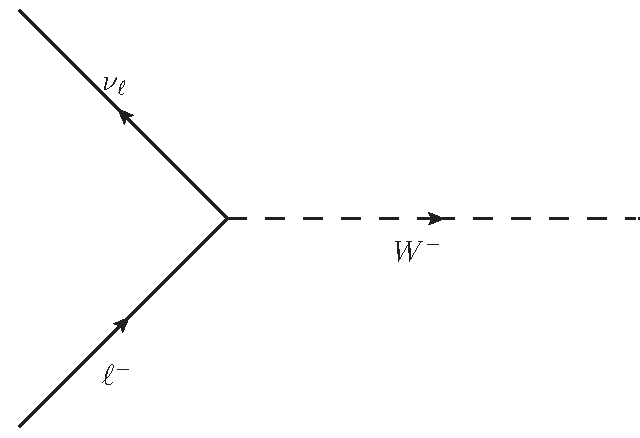
\includegraphics[scale=0.67]{lvtoW.pdf}
\caption{Vértice leptónico fundamental}
\label{Fig:lvtoW}
\end{figure}
%
Aquí un leptón ($e$, $\mu$ y $\tau$) es convertido en su correspondiente neutrino ($\nu_e$, $\nu_{\mu}$ y $\nu_{\tau}$), con la emisión de un $W^{-}$ (o la absorción de $W^{+}$). El proceso de convertir un neutrino en leptones también está permitido y los procesos cruzados incluyen los antileptones. La importancia de las corrientes cargadas en la interacción débil es que permiten cambiar sabor, a diferencia de las demás interacciones que no lo permiten. La regla de Feynmann para el vertice de la interacción débil está dado por:
%
\begin{align*}
\frac{-i g_{W}}{2\sqrt{2}} \gamma^{\mu}(1-\gamma^5)\,,
\end{align*}
%
el factor $2\sqrt{2}$ es por convención,  y el factor ($1-\gamma^5$) hace referencia a que las corrientes débiles solo se acoplan a los leptones levógiros o izquierdos, lo que permite la violación de la simetría de paridad (P).

El acoplamiento de los $W^{\pm}$ se da estrictamente solo para una generación de leptones en particular:
%
\begin{align*}
\begin{pmatrix}\nu_e \\ e \end{pmatrix} \,, &
&\begin{pmatrix}\nu_\mu \\ \mu \end{pmatrix} \,, &
&\begin{pmatrix}\nu_\tau \\ \tau \end{pmatrix} \,.
\end{align*}
%
Los únicos procesos permitidos son $e^{\pm} \to W^{\pm} + \nu_e$, $\mu^{\pm} \to W^{\pm} + \nu_\mu$ y $\tau^{\pm} \to W^{\pm} + \nu_\tau$. Estas restricciones se deben a las leyes de conservación del número electrónico, el número muónico y el número tauónico. El acoplamiento de $W$ a quarks no es tan simple, porque aunque la estructura de generación es similar
%
\begin{align*}
\begin{pmatrix}u \\ d \end{pmatrix}\,, & 
&\begin{pmatrix}c \\ s \end{pmatrix}\,, &
&\begin{pmatrix}t \\ b \end{pmatrix}\,,
\end{align*}
%
las interacciones débiles no está estrictamente restringidas entre generaciones. Debido a que hay interacción entre las partículas de la misma genereación, por ejemplo $d \to u + W^{\pm}$. Pero existen también procesos que combinan generaciones de la forma $s \to u + W^{\pm}$. Si este no fuera el caso, tendríamos tres leyes absolutas de \textquotedblleft conservación del sabor\textquotedblright: la conservación de \textquotedblleft upness-plus-downness\textquotedblright, \textquotedblleft encanto-más-rareza\textquotedblright y \textquotedblleft verdad-más-belleza\textquotedblright análogas a las tres leyes de conservación del número leptónico. De hecho, si así fuera, la partícula extraña más ligera ($K^-$) sería absolutamente estable, y también lo sería el mesón $B$ (la partícula hermosa más liviana); el universo sería un lugar diferente a lo que se conoce.

En 1963, cuando solo se conocían los quarks $u$, $d$ y $s$, el físico Italiano Nicola Cabibbo propuso que los vértices de las interacciones de los quarks debían ser corregidos~\cite{Cabibbo:1963yz}. El vértice $d + \bar{u} \to W^{-}$ debía ser corregido por un factor de $\cos \theta_C$ y el vértice $s + \bar{u} \to W^{-}$ por un factor de $\sin \theta_C$, donde $\theta_C=0.226$ rad es conocido como el ángulo de Cabibbo. Debido a su pequeño valor el vértice $s + \bar{u} \to W^{-}$ está más suprimido que el vértice $b + \bar{u} \to W^{-}$, lo que indica que a diferencia de la interacción débil para leptones, la interacción débil para quarks no prohíbe la interacción entre generaciones~\cite{Cabibbo:1963yz}.
%
\begin{figure}
\centering
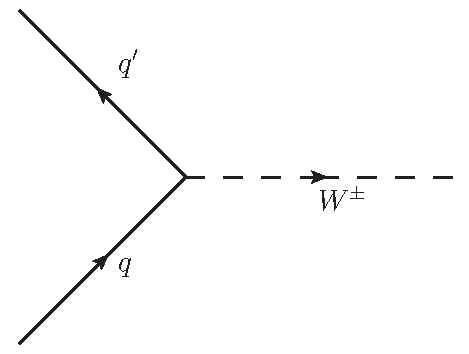
\includegraphics[scale=0.8]{qqtoW}
\caption{Vértices de interacción del bosón $W$ con los quarks. $q$ y $q'$ hacen referencia a los diferentes sabores de quarks ($u$, $d$, $c$, $s$, $b$ y $t$).}
\label{Fig:qqtoW}
\end{figure}
%
La teoría de Cabibbo fue muy exitosa reproduciendo resultados experimentales de una gran cantidad de decaimientos, pero surgió un problema: bajo este modelo la amplitud de decaimiento del mesón $K^{0}$ en un par $\mu^{+}\mu^{-}$ calculada es mucho mayor que los límites experimentales permitidos debido al proceso de la fig.~\ref{Fig:Ktomumu}, el cual es proporcional a $\sin \theta_C \cos \theta_C$. Una solución a este problema fue propuesto por Glashow, Iliopoulos y Maiani (GIM)~\cite{Glashow:1970gm}. Esta solución fue nombrada como mecanismo de GIM, este mecanismo consiste en introducir un cuarto quark (quark $c$), para el cual el vértice de la interacción $c + \bar{d} \to W^{-}$ lleva un factor de $-\sin \theta_C$ y el vértice $c + \bar{s} \to W^{-}$ lleva un factor de $\cos \theta_C$. Debido a este nuevo quark el proceso de la fig.~\ref{Fig:Ktomumu} es cancelado por el diagrama con el mismo proceso intercambiando el $u$ con el $c$, el cual será proporcional a $-\sin \theta_C \cos \theta_C$.

Una simple interpretación de este mecanismo consiste en que los estados físicos de los quarks deben ser $d'$ y $s'$, en lugar de  $d$ y $s$, dados por:
%
\begin{align}\label{Eq:Rot}
\begin{pmatrix}d' \\ s' \end{pmatrix} =& \begin{pmatrix}\cos \theta_C & \sin \theta_C \\ -\sin \theta_C & \cos \theta_C \end{pmatrix}\begin{pmatrix}d \\ s \end{pmatrix} \,.
\end{align}
%
Los bosones $W$ se acoplan a los estados de “Cabibbo rotados”
%
\begin{align*}
\begin{pmatrix}u \\ d' \end{pmatrix}\,, & 
&\begin{pmatrix}c \\ s' \end{pmatrix}\,,
\end{align*}
%
de la misma forma en que se acoplan al par de leptones; donde el acople a las partículas físicas están dados por:
%
\begin{align*}
\begin{pmatrix}u \\ d' \end{pmatrix} =& \begin{pmatrix}u \\ d\cos \theta_C + s \sin \theta_C \end{pmatrix}\,, & 
\begin{pmatrix}c \\ s' \end{pmatrix} =& \begin{pmatrix}c \\ -d\sin \theta_C + s \cos \theta_C \end{pmatrix}\,.
\end{align*}
%
Lo cual implica que $u + \bar{d} \to W^{-}$ lleva un factor de $\cos \theta_C$, $u + \bar{s} \to W^{-}$ lleva un factor de $\sin \theta_C$, $c + \bar{d} \to W^{-}$ lleva un factor de $-\sin \theta_C$ y $c + \bar{s} \to W^{-}$ lleva un factor de $\cos \theta_C$. \footnote{Es de notar que la elección del uso de los quarks tipo down ($d$ y $s$) es una definición arbitraria y por convención. Esto no representa una asimetría física entre quarks de tipo up ($u$ y $c$) y tipo down. Por lo que un desarrollo que  describa los estados de la interacción débil $u'$ y $c'$, en términos de $u$ y $c$ es totalmente equivalente.} El mecanismo GIM se consideraba extravagante debido a que para dar solución a un defecto técnico bastante esotérico, debía introducir un nuevo quark. Además,  para la epoca gran parte de esta teoría estaba aun sin probar. En 1974, los experimentos le dieron la razón a Glashow y compañía con el descubrimiento del quark $c$~\cite{Aubert:1974js}. 
%
\begin{figure}
\centering
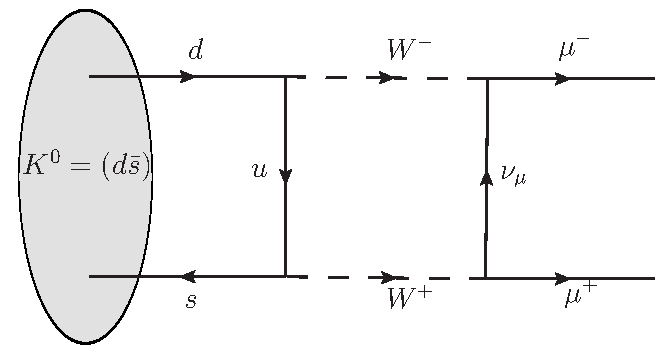
\includegraphics[scale=0.8]{Ktomumu}
\caption{Decaimiento de $K^{0} \to \mu^{+} + \mu^{-}$.}
\label{Fig:Ktomumu}
\end{figure}
%

Para explicar la violación de CP es necesario un número complejo en la matriz de \textquotedblleft rotación\textquotedblright \eqref{Eq:Rot}. Debido a que es posible eliminar las fases complejas de las matrices $2 \times 2$ mediante una redefinición adecuada de las fases de los quarks, no es posible explicar la violación de CP con el mecánismo de GIM. En 1973 antes de que el quark $c$ fuera descubierto, los físicos Japoneses Makoto Kobayashi y Toshihide Maskawa propusieron una explicación a la violación de CP dentro del esquema de Cabibbo-GIM~\cite{Kobayashi:1973fv}. Su propuesta consistía en definir la matriz de rotación $3 \times 3$, generalizando así, la matriz de Cabibbo a la matriz de Cabibbo–Kobayashi–Maskawa (o matriz $V_{\text{CKM}}$). Con esto era posible mantener la fase compleja. Además, se daba cuenta de la existencia de una tercera generación de quarks, conocidas como \textquotedblleft las generaciones de interacción débil\textquotedblright
%
\begin{align*}
\begin{pmatrix}u \\ d' \end{pmatrix}\,, & 
&\begin{pmatrix}c \\ s' \end{pmatrix}\,, &
&\begin{pmatrix}t \\ b' \end{pmatrix}\,,
\end{align*}
%
las cuales están relacionadas con  los estados de quarks físicos mediante la matriz $V_{\text{CKM}}$
%
\begin{align*}
\begin{pmatrix}d' \\ s' \\ b' \end{pmatrix} =& 
\begin{pmatrix}V_{ud} & V_{us} & V_{ub} \\ V_{cd} & V_{cs} & V_{cb} \\ V_{td} & V_{ts} & V_{tb} \end{pmatrix}
\begin{pmatrix}d \\ s \\ b \end{pmatrix}
\end{align*}
%
donde $V_{q q'}$ hace referencia a las mezclas entre el quark $q$ y el $q'$. Por ejemplor, $V_{ud}$ hace referencia a la mezcla $u + \bar{d} \to W^{-}$. Por lo que hay nueve entradas en la matriz $V_{\text{CKM}}$, pero no todos son parámetros independientes, ya que es posible llevar esta matriz a su forma canonica, en esta forma dicha matriz dependerá de los ángulos de Cabibbo generalizados ($\theta_{12}$, $\theta_{13}$ y $\theta_{23}$) y una fase $\delta$
%
\begin{align*}
V_\text{CKM} =& 
\begin{pmatrix}
c_{12} c_{13} & s_{12} c_{13} & s_{13} e^{-i\delta} \\ 
-s_{12} c_{23} - c_{12} s_{23} s_{13} e^{i\delta} & c_{12} c_{23} - s_{12} s_{23} s_{13} e^{i\delta} & s_{23} c_{13} \\ 
s_{12} s_{23} - c_{12} c_{23} s_{13} e^{i\delta} & -c_{12} s_{23} - s_{12} c_{23} s_{13} e^{i\delta} & c_{23} c_{13} 
\end{pmatrix}\,,
\end{align*}
%
donde $c_{ij} = \cos \theta_{ij}$ y $s_{ij} = \sin \theta_{ij}$. Si hacemos $\theta_{23} = \theta_{13} = \delta = 0$ y $\theta_{12} = \theta_C$, la tercera generación no se mezcla con las otras dos y es posible recuperar la teoría de  Cabibbo-GIM. Sin embargo, debido al decaimiento del mesón $B^{-}$($\bar{u}b$) se sabe que la tercera familia se mezcla a la primera, aunque esta mezcla debe ser bastante pequeña para poder explicar el éxito del esquema Cabibbo-GIM original. Además, debido a que el ME no ofrece ninguna predicción sobre los valores de la matriz  $V_{\text{CKM}}$ solo se conocen los valores de los elementos de la matriz mediante los diferentes  experimentos diseñados para medir éstos. Las magnitudes y su precisión están dados por:
%
\begin{align*}
V_{\text{CKM}} =& 
\begin{pmatrix}
0.97427\pm 0.00015 & 0.22534\pm 0.00065 & 0.00351^{+0.00015}_{-0.00014} \\ 
0.22520\pm 0.00065 & 0.97344\pm 0.00016 & 0.0412^{+0.0011}_{-0.0005} \\ 
0.00867^{+0.00029}_{-0.00031} & 0.0404^{+0.0011}_{-0.0005} & 0.999146^{+0.000021}_{-0.000046}
\end{pmatrix}\,,
\end{align*}
%
y la fase tiene un valor de $\delta = 1.20 \pm 0.08$. La mezcla de la tercera familia (los elementos  de la tercera fila y columna fuera de la diagonal) con las demás resulta ser muy pequeña, debido a la larga vida del mesón $B$ ($10^{-12}$ seg)~\cite{Beringer:1900zz}.


\section{Universalidad}

En el ME de partículas, cada fermión tiene tres copias idénticas, siendo la masa la única diferencia entre ellas. A cada una de dichas copias se les conoce como familias o generaciones de fermiones. Debido a esto no es posible diferenciar entre una familia u otra en procesos físicos en los que masa no sea un parámetro relevante. Esta propiedad emergente del ME se conoce como universalidad.

Para comprobar la universalidad del bosón $W$ es necesario determinar los anchos de decaimiento, por lo que es necesario conocer el lagrangiano de interacción. El Lagrangiano que describe la interacción de los fermiones al bosón $W$ es:
%
\begin{align}\label{Eq:LagW}
\mathcal{L} = \frac{g_W}{\sqrt{2}} (\overline{q'} {W}_{\mu}^{-}  \gamma ^{\mu} V_{\text{CKM}} P_{L} q + \overline{\nu_{\ell}} {W}_{\mu}^{-} \gamma ^{\mu} P_{L} \ell^{-}) + \text{h.c.}\,,
\end{align}
%
donde $P_{L} = (1 - \gamma_5)/2$ es el proyector izquierdo, $q$ y $q'$ hacen referencia a los quarks ($u$, $d$, $c$, $s$, $b$ y $t$), $\ell$ hace referencia a los diferentes leptones ($e$,$\mu$ y $\tau$).

Debido a que el quark $t$ es más pesado que el bosón $W$, los decaimientos $W \to t d$, $W \to t s$ y $W \to t b$ no son permitidos, por lo que el ancho total de decaimiento del $W$ sería dividido en dos partes, las cuales dependen del producto de estados finales
%
\begin{align}\label{Eq:AnchoW}
\Gamma_{tot} (W) = \sum_{q q^{\prime}}\Gamma(W \to q \bar{q}^{\prime}) + \sum_{\ell} \Gamma(W \to \ell \bar{\nu_{\ell}})\,,
\end{align}
%
donde $q = u$, $c$, $q' = d$, $s$, $b$ y $\ell = e$, $\mu$, $\tau$. Para efectos prácticos se considera que todos los quarks son no masivos excepto el quark $t$, ya que la masa del $W$ es mucho mayor que la masa de los demás quarks. Los anchos de decaimiento para los miembros derechos de la ecuación \eqref{Eq:AnchoW} están dados por:
%
\begin{align}\label{Eq:Gamma}
\Gamma(W \to q \bar{q'}) =& \frac{|V_{\text{CKM}qq'}|^2 g_W^2}{16 \pi} M_{W} \approx 0.6757 |V_{\text{CKM}qq'}|^2 \text{ GeV}\,, \\
\Gamma(W \to \ell \bar{\nu_{\ell}}) =& \frac{g_W^2}{48 \pi} M_{W}\approx 0.2252 \text{ GeV}\,,
\end{align}
%
donde $g_W^2 = 8M^2_{W}G_F / \sqrt{2}$ y $V_{\text{CKM}qq'}$ son las respectivas entradas de la matriz $V_{\text{CKM}}$, $M_{W}$ es la masa del bosón $W$ y $G_F$ es la constante de Fermi. El ancho total de decaimiento para el bosón $W$ es:
%
\begin{align}
\Gamma_{tot}(W) =& \frac{g_W^2}{16 \pi}\left[\sum_{q q^{\prime}} |V_{\text{CKM}qq'}|^2 + 1 \right] M_{W}\,.
\end{align}
%
Haciendo la suma sobre la CKM, tenemos \begin{align*}
\sum_{q q^{\prime}} |V_{\text{CKM}qq'}|^2 = 1.99999 \approx 2.0 \,,
\end{align*} por lo que la amplitud total de decaimiento toma la forma:
%
\begin{align}
\Gamma_{tot}(W) =& \frac{3 g_W^2}{16 \pi} M_{W} \approx 2.094 \text{GeV}\,,
\end{align}
%
y los branching son iguales a
%
\begin{align}\label{Eq:Branching}
B(W \to \ell \nu_{\ell}) =& \frac{1}{9} \approx 11.1\% \,, & 
B(W \to \text{Hadrones})= \sum_{q q^{\prime}} B(W \to q \bar{q'}) =& \frac{2}{3} \approx 66.6\%\,.
\end{align}
%
Lo cual concuerda con los resultados experimentales~\cite{Beringer:1900zz}
\begin{align*}
B(W \to \ell \nu_{\ell}) =& (10.80 \pm 0.09)\%\,, & B(W \to \text{Hadrones})= \sum_{q q^{\prime}} B(W \to q \bar{q'}) =& (67.60 \pm 0.27)\%\,.
\end{align*} 
%
Debido a que en las desintegraciones débiles de alta energía los efectos de la masa son despreciables en la Eq. \eqref{Eq:Gamma}, el bosón $W$ debe de decaer con igual probabilidad a las diferentes familias de leptones. Esta propiedad emergente se le conoce como la Universalidad Leptónica (UL), la cual implica que los bosones vectoriales se acoplan por igual a las tres familias de leptones. 
En particular, las mediciones de los decaimientos $b \rightarrow c \ell \nu$ para diferentes leptones de estado final, pueden ser utilizadas probar la UL con una gran precisión, dado la cancelación de muchas fuentes de incertidumbres teóricas que ocurren en relaciones, tales como:
\begin{align}
R(D^{(*)}) = \frac{\Gamma(B \rightarrow D^{(*)} \tau \nu)}{\Gamma(B \rightarrow D^{(*)} \ell \nu)}\,,
\end{align}
con $\ell = e$ o $\mu$. El ME predice que los valores para dichos procesos deben ser $R(D) = 0.298 \pm 0.003$ y $R(D^*) = 0.255 \pm 0.004 $. Adicionalmente, las mediciones de la razón
\begin{align}
R_K = \frac{\Gamma(B \rightarrow K \mu ^+ \mu ^-)}{\Gamma(B \rightarrow K e^+ e^-)}\,,
\end{align}
deben respetar la UL y por lo tanto el valor predicho por el ME es $R_K = 1.0$~\cite{Beringer:1900zz}.
